\documentclass[reprint, english, nofootinbib]{revtex4-2}

\usepackage{graphicx}
\usepackage{subfig}
\usepackage[colorlinks=true,urlcolor=blue,citecolor=blue]{hyperref}
\usepackage{physics}
\usepackage{amsmath}
\usepackage{amssymb}
\usepackage{amsbsy}
%\usepackage{bbold}
\usepackage{subfig}

\usepackage{blindtext}
\usepackage{tikzducks}
\usepackage{listings}

\graphicspath{{../figs/}}

\begin{document}
\title{Regression analysis and resampling methods}
\author{Nicholas Karlsen}
\affiliation{University of Oslo}
\author{Thore Espedal Moe}
\affiliation{University of Oslo}
\date{\today}

\begin{abstract}
    \noindent
   In this paper we aim to explore the application of three distinct regression methods to both a sampling of the Franke function, as well as a set of terrain data. We utilize the ordinary-least-square (OLS) regression, Ridge regression and LASSO regression along with bootstrap and k-fold cross-validation re-sampling techniques in order to create and asses predictive polynomial models. We analyze the performance of the different regression models on the two data sets, with the ultimate goal of determining the best regression method and the best predictive polynomial model for each data set.
\end{abstract}

\maketitle

\section{Introduction}
    \noindent
    In essence, Linear Regression is the process of taking points from a function, or a set of measurements, and mapping them to coordinates in a chosen basis in order to create an approximation, or model, of the original dataset.
    % Maybe not original dataset, but underlying function/process/phenomena?
     That is, from a limited set of data try to infer a functional relationship between some chosen prediction variables and the measured/sampled responses, and use this functional relationship to predict new data points in the domain. Typically, one is either interested in extracting the functional relationship between the measured responses and the prediction variables in order to say something about the relative importance of the conjectured predictors; or one wants to create a "best possible" predictive map of the (mostly unmeasured) response variables as a function of the (mostly unmeasured) prediction variables. In both cases what one really wants is a some form of optimal mapping from prediction variables to response variables, and that can be provided by the use of linear regression methods.
     
     Obviously, this way of doing predictions and inferences has an enormous selection of possible applications. In this paper we investigate two illustrative and similar applications: The reconstruction of the Franke function from sampled values, and the (re-)construction of an elevation map from a donwsampled set of terrain data. In a way, our data sets are "low-resolution images" of the Franke function and the terrain. Our goal is then to find the best possible "high-resolution images" by using different regression methods and resampling techniques on the sampled data, using tow-dimensional polynomials as basis functions. In other words, we want to find the most faithful recreation of the original terrain data and the Franke function, in the basis of two-dimensional polynomials.
     
     We begin with a theoretical discussion of the regression and resampling methods that will be used, as well as some comments on the significance of the so-called Bias-Variance-Tradeoff in the context of linear regression. We then proceed to investigate the application of ordinary-least-squares (OLS), Ridge regression and LASSO regression to samplings of the Franke function. We use k-fold cross-validation to assess the mean-squared-error (MSE) of our different models, and we use bootstrap resampling in order to estimate the bias and variance of our models. We discuss the influence of the number of points sampled, the polynomial degree we try to fit, the values of the hyper-parameter lambda for the Ridge and LASSO regressions and the presence/absence of noise in our samplings. Afterwards we will move on to the terrain data, where we perform much of the same analysis as for the Franke function. We then try to evaluate which regression methods perform the best for different use cases, and which resulting models might be considered the 'best'.
     
     
\section{Theory}
    \subsection{Linear Regression}
        \noindent
        Consider a set of data points $\{(x_1, y_i), \dots, (x_N, y_N)\}$ which we wish to fit to some linear model $\pmb{\tilde y}(\pmb \beta)$ where $\pmb\beta$ is a vector containing the free parameters of the model. The model $\pmb{\tilde y}$ will then be related to the true data points $\pmb y$ by
        \begin{equation}
            \pmb y = \pmb{\tilde y}(\pmb\beta) + \pmb\varepsilon
        \end{equation}
        where $\pmb\varepsilon = (\varepsilon_1, \dots, \varepsilon_N)$ represents the error of the model. The aim of Linear regression models is thus to find the optimal parameters $\pmb\beta$ such that not only the error of the model on some particular dataset is minimized, but also the error of the model applied to different data sets sampled in the same domain is minimized such that we may use our model to make predictions about new datasets.

        \subsubsection{The Design Matrix}
            \noindent
            When constructing a model, we first have to chose a set of basis functions. A popular choice for which is $\mathbb P_n$, which models a wide range of different phenomena and is also the choice we will make for this paper. But in principle, any set of linear basis functions may be chosen.
            For a single variate polynomial, a model would then take the form
            \begin{equation}
                \tilde y (x) = \beta_0 + \beta_1 x+ \dots + \beta_n x^n
            \end{equation}
            When trying to find the optimal $\pmb \beta$, a useful construct is the so-called Design Matrix, which for a polynomial basis takes the form
            \begin{equation}
                \textup{X} = \qty[
                \begin{matrix}
                    1 & x_1 & \dots & x_1^n \\
                    1 & x_2 & \dots & x_2^n \\
                    \vdots & \vdots & \vdots & \vdots \\
                    1 & x_N & \dots & x_N^n
                \end{matrix}
                ]
            \end{equation}
            where we see that entry $\textup{X}_{ij}$ contains the $x_i$ data point evaluated in the $j$-th basis function. This matrix has the particularly useful property that we may then multiply it with $\pmb \beta$ to obtain the corresponding set of predictions $\pmb{\tilde y}$ like
            \begin{equation}
                \pmb{\tilde y} = \textup{X}\pmb \beta
            \end{equation}
            leaving us with a linear algebra problem to solve in finding the $\pmb\beta$ which optimizes $\pmb{\tilde y}$.

            This also extends directly to multivariate cases where we have more than one independent variable. In particular for two dimensional polynomials, our choice of basis for this article, we have that an $n$-th degree polynomial is constructed by all permutations of $x^p y^q$ where $p+q \leq n$ which means that the total number of predictors for degree $n$ is given by
            \begin{equation}
                \qty(
                \begin{matrix}
                    2 + n \\ n
                \end{matrix}
                )
                =\frac{(2+n)!}{n!(2+n-n)!} = \frac{(n+1)(n+2)}{2}
            \end{equation}

        \subsubsection{Model assessment}
            \noindent
            Once we have constructed a model, we a also need a way to quantitatively evaluate its performance. Here, we will focus on two statistical measures; First, we have the \textit{mean squared error} (MSE) defined as
            \begin{equation}
                \textup{MSE}(\pmb y, \pmb{\tilde y}) = \frac{1}{n}\sum_i \qty(y_i - \tilde y_i)^2
            \end{equation}
            which as the name suggests is a measure of the mean square distance the model $\pmb{\tilde y}$ has from the data set $\pmb y$. We also have the \textit{coefficient of determination}, defined as
            \begin{equation}
                \textup{R}^2(\pmb y, \tilde{\pmb{y}}) = 1 -
                \frac{\sum_i(y_i - \tilde y_i)^2}{\sum_i \qty(y_i - \mathbb E\qty[\pmb y])^2}
            \end{equation}
            which loosely speaking is a measure of well the proposed model predicts the variance of the data set, where R$^2 = 1$ corresponds to a perfect fit and R$^2 < 1$ an increasingly worse fit.

            A particularly important point to make when considering these measures is that they will both generally favor increasingly higher degree polynomials when looking at some particular data set. Whilst yielding good MSE \& R$^2$ scores this leads to over-fitting, where the model becomes too specialized to one particular sample which means that the overall predictive capabilities of the model actually decreases. We will look closer at the details of this in a later section. For now, we simply note that this problem motivates us to split our data sets into training and test sets. Where we train our model using the training set, and subsequently validate the model by computing the MSE \& R$^2$ scores on the test sets. Thus, if our model becomes too specialized to the training set, this will lower MSE R$^2$ scores in the test set, giving us a much better indication on the predictive capabilities of our model.

        \subsubsection{Ordinary Least Squares}
            \noindent
            In ordinary least squares (OLS), we aim to find an optimal set of parameters $\pmb{\hat\beta} = [\hat\beta_0, \dots, \hat\beta_n]^T$ such that the $L^2$ norm $\norm{\pmb y - \textup{X}\pmb{\beta}}_2$ is minimal, with the $L^2$ norm being induced by the inner product
            \begin{equation}
                \norm{\pmb u}_2^2 = \sum_i u_i^2 = \pmb u^T \pmb u
            \end{equation}
            This defines the cost function for OLS, which may be written as
            \begin{equation}
                C_{OLS}(\pmb \beta)
                = \qty(\pmb y - \textup{X}\pmb \beta)^T(\pmb y - \textup{X}\pmb \beta)
            \end{equation}
            In order to find the minima, we differentiate wrt to $\pmb\beta$ and assert that $\partial_{\pmb\beta}C_{OLS} = 0$ for the optimal predictor. Taking the partial derivative yields
            \begin{align}
                \begin{split}
                \pdv{\pmb\beta}C_{OLS}(\pmb\beta) = -2\textup{X}^T\qty(\pmb y - \textup X\pmb \beta)
                \end{split}
            \end{align}
            We assert this is zero at the minima, which yields
            \begin{equation}
                \textup{X}^T\pmb y = \textup{X}^T\textup{X}\pmb\beta
            \end{equation}
            then taking the inverse of $\textup{X}^T\textup{X}$ on both sides then gives the optimal $\pmb\beta$ as
            \begin{equation}\label{eqn:OLS optimal beta}
                \hat{\pmb \beta}_{\textup{OLS}} = (\textup{X}^T\textup{X})^{-1}\textup{X}^T\pmb y
            \end{equation}
            which mathematically is the best projection of the data-points to our model. However, this may not actually yield the best predictive model. OLS may suffer from over-fitting to the particular sample, and will therefore not always perform very well on new data points for which the model has not been trained. As such, we instead look at alternate regression methods with additional turning parameters which allow us to account for the variance between different sets of data as to yield a model with better predictive abilities compared to the OLS.

        \subsubsection{Ridge Regression}
            \noindent
            One such method is the Ridge regression where we instead try to minimize $\norm{\pmb y - \textup{X}\pmb \beta}_2 + \lambda\norm{\pmb \beta}_2$, from which we define our cost function as
            \begin{equation}
                C_{R}(\pmb \beta)
                = (\pmb y - \textup{X}\pmb\beta)^T(\pmb y - \textup{X}\pmb\beta)
                + \lambda \pmb\beta^T\pmb\beta
            \end{equation}
            Similar for what we did for OLS, we take the partial derivative wrt. $\pmb \beta$, where the only difference in finding the minima resides in the additional term
            \begin{equation}
                \pdv{\pmb \beta} \lambda \pmb\beta^T\pmb\beta = 2\lambda\pmb\beta
            \end{equation}
            if we again assert that the optimal $\pmb\beta$ is given by $\partial_{\pmb\beta}C_R(\pmb\beta)$ and rearrange we get
            \begin{equation}
                \pmb{\hat\beta}_R = \qty(\textup{X}^T\textup{X}  + \lambda)^{-1}\textup{X}^T\pmb{\tilde y}
            \end{equation}
            As the optimal $\beta$ for Ridge regression.
            So we see that the only difference between OLS and Ridge regression is the addition of the "penalty" parameter $\lambda$ to the $L^2$ norm of the coefficients $\pmb{\beta}$. The main point of introducing this parameter is to reduce the variance of the regression coefficients $\pmb{\beta}$. It introduces a constraint on the allowable values of $\pmb{\beta}$, which means that the method no longer is unbiased. The aim is that the reduction of the variance outweighs the increase of the method's bias, leading to an overall lower test error, cf. the later discussion of the Bias-Variance Trade-off. As a techincal note, during our computations we center our response-variable and scale plus center our predictors. This has the effect of removing the constant column in the design, so that penalty term doesn't apply to $\beta_{0}$.
            
            
        \subsubsection{LASSO Regression}
            The cost function for the \textit{least absolute shrinkage and selection operator} (LASSO) method is defined as
            \begin{equation}
                C_L(\pmb \beta) =
                \norm{\pmb y - \textup{X}\pmb{\beta}}_2^2
                + \lambda\norm{\pmb{\beta}}_1
            \end{equation}
            Which as opposed to OLS and Ridge has no analytical solution for finding the optimal $\pmb \beta$, which is instead found by optimization methods such as gradient descent. The specifics of this is beyond the scope of this article, and we will simply use the existing libraries provided by scikit-learn~\cite{scikit-learn} to perform the regression.

            Qualitatively the Lasso method is distinguished from the Ridge regression by how the norm of $\pmb{\beta}$ is penalized. While the Ridge regression applies the penalty to the $L^2$ norm, the Lasso aims to shrink the $L^1$ norm. Two important consequences arise from this: firstly, it is no longer possible to obtain a closed-form solution to the minimization problem; secondly, the regression coefficients may be shrunk far more unevenly. In contrast to the Ridge regression, Lasso regression may shrink individual $\beta_{i}$ toward zero. This is an extremely useful property of the method, since it allows unimportant predictors to be identified and discarded. The drawback, of course, is that the bias of the Lasso method is expected to exceed the bias of the Ridge method. Once again, by  centering we remove the constant column from the design matrix to avoid penalizing the constant term through $\beta_{0}$.

    \subsection{Singular Value Decomposition}
        \noindent
        Consider an $m\times n$ matrix $\textup X$ of rank $r$. The singular values of $\textup X$ are then defined as the root of the eigenvalues of the diagonal matrix $\textup X^T\textup X$. We may also express $\textup X$ in the so-called singular value decomposition (SVD)
        \begin{equation}
            \textup X = \textup{U}\Sigma\textup{V}^T
        \end{equation}
        where $\textup{U, V}$ are unitary matrices and
        \begin{equation}
            \Sigma =
            \qty[
            \begin{matrix}
                D & \dots & 0 \\
                \vdots & \ddots & \vdots \\
                0 & \dots & 0
            \end{matrix}
            ]
        \end{equation}
        an $m\times n$ matrix, where the matrix $\textup D$ is a diagonal $r \times r$ matrix containing the singular values of $\textup X^T \textup X$
        \begin{equation}
            D = \qty[
            \begin{matrix}
                \sigma_1 & \dots & 0 \\
                \vdots & \ddots & \vdots \\
                0 & \dots & \sigma_n
            \end{matrix}
            ]
        \end{equation}
        which by convention is ordered such that $\sigma_1 \geq \dots \geq \sigma_n$.

        \subsubsection{Application to OLS}
            We may use the SVD to re-express the expression for $\hat{\pmb \beta}$ in OLS given by Eqn.~\ref{eqn:OLS optimal beta}
            by writing
            \begin{equation}
                \textup{X}^T\textup{X} = \qty(\textup{U}\Sigma\textup{V}^T)^T\qty(\textup{U}\Sigma\textup{V}^T)
                = \textup{V}\Sigma^T\textup{U}^T\textup{U}\Sigma\textup{V}^T
            \end{equation}
            Since $\textup{U}$ is unitary, it follows that $\textup{U}^T\textup{U} = \mathbb I$, further we have that $\Sigma^T = \Sigma$ since it is a diagonal matrix. We therefore end up with
            \begin{equation}
                \textup{X}^T\textup{X} = \textup{V}\Sigma^2\textup{V}^T
            \end{equation}
            inserting this into Eqn.~\ref{eqn:OLS optimal beta} gives us
            \begin{equation}
                \pmb{\hat{\beta}}_{\textup{OLS}} = \qty(\textup{V}\Sigma^2\textup{V}^T)^{-1} \textup{V}\Sigma\textup{U}^T\pmb{y}
            \end{equation}
            This gives an alternate way of solving the OLS problem, which becomes particularly useful in situations where we have a large amount of data sampled from a relatively small domain, increasing the chance of X having linearly dependent columns which in turns leads to X, and by extension X$^T$X no longer being invertible.
    \subsection{Re-sampling}
        \noindent
        Re-sampling methods are ways in which we can generate new statistics from our existing data, which as the name suggests implies sampling new data sets from our already existing data. By doing so, we may gain new insights about our data which may not be available through regular analysis, particularly in situations where we are limited by the number of data points.

        Here, we will focus on two of many such techniques.

        \subsubsection{Cross Validation}
            \noindent
            In the cross-validation re-sampling method, we split our data set $S$ into $k$ equally sized subsets $s_1, \dots, s_k$.
            We then for each $i = 1,\dots, k$ assign the $i$-th subset as the test set and the remaining $k-1$ subsets as the training set and compute the statistics in the usual way. Then at the end, we compute the mean value of the $k$ sets of statistics. A visual representation of this process can be seen in Fig.~\ref{fig: Cross Validation}.
            \begin{figure}[h!tb]
                \center
                \vspace{5mm} % To avoid touching the preceding text
                \tikzset{every picture/.style={line width=0.75pt}} %set default line width to 0.75pt

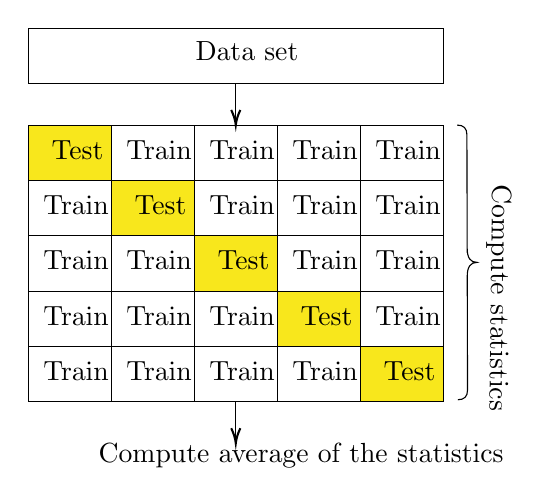
\begin{tikzpicture}[x=0.5pt,y=0.5pt,yscale=-1,xscale=1]
%uncomment if require: \path (0,487); %set diagram left start at 0, and has height of 487

%Shape: Rectangle [id:dp9628831478307318]
\draw   (90,20) -- (390,20) -- (390,60) -- (90,60) -- cycle ;
%Shape: Rectangle [id:dp40247556319098454]
\draw   (150,90) -- (210,90) -- (210,130) -- (150,130) -- cycle ;
%Straight Lines [id:da38673279994063514]
\draw    (240,60) -- (240,88) ;
\draw [shift={(240,90)}, rotate = 270] [color={rgb, 255:red, 0; green, 0; blue, 0 }  ][line width=0.75]    (10.93,-3.29) .. controls (6.95,-1.4) and (3.31,-0.3) .. (0,0) .. controls (3.31,0.3) and (6.95,1.4) .. (10.93,3.29)   ;
%Shape: Brace [id:dp44265578721237586]
\draw   (400.5,288.5) .. controls (405.17,288.49) and (407.49,286.15) .. (407.48,281.48) -- (407.28,199.23) .. controls (407.27,192.56) and (409.59,189.23) .. (414.26,189.22) .. controls (409.59,189.23) and (407.25,185.9) .. (407.23,179.23)(407.24,182.23) -- (407.03,96.98) .. controls (407.02,92.31) and (404.68,89.99) .. (400.01,90) ;
%Shape: Rectangle [id:dp6086176363319614]
\draw  [fill={rgb, 255:red, 248; green, 231; blue, 28 }  ,fill opacity=1 ] (90,90) -- (150,90) -- (150,130) -- (90,130) -- cycle ;
%Shape: Rectangle [id:dp6253670891530648]
\draw   (210,90) -- (270,90) -- (270,130) -- (210,130) -- cycle ;
%Shape: Rectangle [id:dp012463141021535118]
\draw   (270,90) -- (330,90) -- (330,130) -- (270,130) -- cycle ;
%Shape: Rectangle [id:dp03635717517805359]
\draw   (330,90) -- (390,90) -- (390,130) -- (330,130) -- cycle ;
%Shape: Rectangle [id:dp6139521323150046]
\draw   (90,130) -- (150,130) -- (150,170) -- (90,170) -- cycle ;
%Shape: Rectangle [id:dp2734748607023023]
\draw   (210,130) -- (270,130) -- (270,170) -- (210,170) -- cycle ;
%Shape: Rectangle [id:dp7416160208443594]
\draw   (270,130) -- (330,130) -- (330,170) -- (270,170) -- cycle ;
%Shape: Rectangle [id:dp04965387626199025]
\draw   (330,130) -- (390,130) -- (390,170) -- (330,170) -- cycle ;
%Shape: Rectangle [id:dp36390369464546923]
\draw   (90,170) -- (150,170) -- (150,210) -- (90,210) -- cycle ;
%Shape: Rectangle [id:dp0583337342908441]
\draw   (150,170) -- (210,170) -- (210,210) -- (150,210) -- cycle ;
%Shape: Rectangle [id:dp7518796244751725]
\draw   (270,170) -- (330,170) -- (330,210) -- (270,210) -- cycle ;
%Shape: Rectangle [id:dp8731512433065419]
\draw   (330,170) -- (390,170) -- (390,210) -- (330,210) -- cycle ;
%Shape: Rectangle [id:dp3374950674483356]
\draw   (90,210) -- (150,210) -- (150,250) -- (90,250) -- cycle ;
%Shape: Rectangle [id:dp2425800253901771]
\draw   (150,210) -- (210,210) -- (210,250) -- (150,250) -- cycle ;
%Shape: Rectangle [id:dp9764918971023423]
\draw   (210,210) -- (270,210) -- (270,250) -- (210,250) -- cycle ;
%Shape: Rectangle [id:dp3030426321919574]
\draw   (330,210) -- (390,210) -- (390,250) -- (330,250) -- cycle ;
%Shape: Rectangle [id:dp08910405765909535]
\draw   (90,250) -- (150,250) -- (150,290) -- (90,290) -- cycle ;
%Shape: Rectangle [id:dp3282550386553066]
\draw   (150,250) -- (210,250) -- (210,290) -- (150,290) -- cycle ;
%Shape: Rectangle [id:dp25498660930064765]
\draw   (210,250) -- (270,250) -- (270,290) -- (210,290) -- cycle ;
%Shape: Rectangle [id:dp08541585559965792]
\draw   (270,250) -- (330,250) -- (330,290) -- (270,290) -- cycle ;
%Shape: Rectangle [id:dp19772098788401882]
\draw  [fill={rgb, 255:red, 248; green, 231; blue, 28 }  ,fill opacity=1 ] (150,130) -- (210,130) -- (210,170) -- (150,170) -- cycle ;
%Shape: Rectangle [id:dp01839862708870832]
\draw  [fill={rgb, 255:red, 248; green, 231; blue, 28 }  ,fill opacity=1 ] (210,170) -- (270,170) -- (270,210) -- (210,210) -- cycle ;
%Shape: Rectangle [id:dp11813630833655397]
\draw  [fill={rgb, 255:red, 248; green, 231; blue, 28 }  ,fill opacity=1 ] (270,210) -- (330,210) -- (330,250) -- (270,250) -- cycle ;
%Shape: Rectangle [id:dp9995560009248317]
\draw  [fill={rgb, 255:red, 248; green, 231; blue, 28 }  ,fill opacity=1 ] (330,250) -- (390,250) -- (390,290) -- (330,290) -- cycle ;
%Straight Lines [id:da24602633489740156]
\draw    (240,290) -- (240,318) ;
\draw [shift={(240,320)}, rotate = 270] [color={rgb, 255:red, 0; green, 0; blue, 0 }  ][line width=0.75]    (10.93,-3.29) .. controls (6.95,-1.4) and (3.31,-0.3) .. (0,0) .. controls (3.31,0.3) and (6.95,1.4) .. (10.93,3.29)   ;

% Text Node
\draw (105,99) node [anchor=north west][inner sep=0.75pt]   [align=left] {Test};
% Text Node
\draw (159,99) node [anchor=north west][inner sep=0.75pt]   [align=left] {Train};
% Text Node
\draw (209,28) node [anchor=north west][inner sep=0.75pt]   [align=left] {Data set};
% Text Node
\draw (441.01,131.27) node [anchor=north west][inner sep=0.75pt]  [rotate=-90.74] [align=left] {Compute statistics};
% Text Node
\draw (139,318) node [anchor=north west][inner sep=0.75pt]   [align=left] {Compute average of the statistics};
% Text Node
\draw (219,99) node [anchor=north west][inner sep=0.75pt]   [align=left] {Train};
% Text Node
\draw (279,99) node [anchor=north west][inner sep=0.75pt]   [align=left] {Train};
% Text Node
\draw (339,99) node [anchor=north west][inner sep=0.75pt]   [align=left] {Train};
% Text Node
\draw (99,139) node [anchor=north west][inner sep=0.75pt]   [align=left] {Train};
% Text Node
\draw (219,139) node [anchor=north west][inner sep=0.75pt]   [align=left] {Train};
% Text Node
\draw (279,139) node [anchor=north west][inner sep=0.75pt]   [align=left] {Train};
% Text Node
\draw (339,139) node [anchor=north west][inner sep=0.75pt]   [align=left] {Train};
% Text Node
\draw (99,179) node [anchor=north west][inner sep=0.75pt]   [align=left] {Train};
% Text Node
\draw (159,179) node [anchor=north west][inner sep=0.75pt]   [align=left] {Train};
% Text Node
\draw (279,179) node [anchor=north west][inner sep=0.75pt]   [align=left] {Train};
% Text Node
\draw (339,179) node [anchor=north west][inner sep=0.75pt]   [align=left] {Train};
% Text Node
\draw (99,219) node [anchor=north west][inner sep=0.75pt]   [align=left] {Train};
% Text Node
\draw (159,219) node [anchor=north west][inner sep=0.75pt]   [align=left] {Train};
% Text Node
\draw (219,219) node [anchor=north west][inner sep=0.75pt]   [align=left] {Train};
% Text Node
\draw (339,219) node [anchor=north west][inner sep=0.75pt]   [align=left] {Train};
% Text Node
\draw (99,259) node [anchor=north west][inner sep=0.75pt]   [align=left] {Train};
% Text Node
\draw (159,259) node [anchor=north west][inner sep=0.75pt]   [align=left] {Train};
% Text Node
\draw (219,259) node [anchor=north west][inner sep=0.75pt]   [align=left] {Train};
% Text Node
\draw (279,259) node [anchor=north west][inner sep=0.75pt]   [align=left] {Train};
% Text Node
\draw (165,139) node [anchor=north west][inner sep=0.75pt]   [align=left] {Test};
% Text Node
\draw (225,179) node [anchor=north west][inner sep=0.75pt]   [align=left] {Test};
% Text Node
\draw (285,219) node [anchor=north west][inner sep=0.75pt]   [align=left] {Test};
% Text Node
\draw (345,259) node [anchor=north west][inner sep=0.75pt]   [align=left] {Test};


\end{tikzpicture}

                \caption{\label{fig: Cross Validation}Visual representation of $k$-fold cross-sampling for $k=5$}
            \end{figure}
            When doing cross-validation, typical choices of $k$ are $5$ and $10$ \cite{hastie}. Which one is better will depend on how the error scales with the size of the training set, as such, choosing a suitable $k$ requires some analysis.
            The cross-validation re-sampling provides a good estimate for the mean error of our estimates.
            \begin{itemize}
                \item Discuss this in more detail $\rightarrow\Delta Err$ wrt to number of data points
            \end{itemize}
        \subsubsection{Bootstrap}
            \noindent
            In the bootstrap re-sampling method, we sample our data set $S = \{s_1, \dots s_N\}$ $N$-number of times, in particular, we allow sampling the same $s_i$ multiple times. In this way, we generate new datasets in which some points are under-weighted and others overweighted with respect to the original dataset $S$. Loosely speaking, the concept corresponds to evenly sampling the ensemble of all possible input data sets to our regression method, in order to estimate the variance and expectation values of our model predictions over the ensemble. The idea is that if our training set representatively covers the domain of inputs, each re-sampled regression computation will give a certain prediction $\pmb{\tilde{y}_{B}}$ and these $\pmb{\tilde{y}_{B}}$ will appear with a frequency corresponding to their  underlying probability distribution. When we later try to compute statistics of the predictions, we will then be able to use point-estimators on the computed $\pmb{\tilde{y}_{B}}$ to obtain estimates of, for instance, the variance of the predictions or the mean value of the predictions over the ensemble of all possible inputs in the domain spanned by our data.

    \subsection{The Bias-Variance Trade-off}
        %%%NICHOLAS' DRAFT START
        % Consider a set of data $S$, sampled from some domain $D$ and two separate models. $\tilde{\pmb y}_s(x)$, a simple model with only a few degrees of freedom and $\tilde{\pmb y}_c(x)$, a more complicated model with many degrees of freedom.

        % When fitting $\pmb{\tilde y}_s(x)$ to the sample $S$ we only have a few degrees of freedom to tune in order to fit the data, resulting in a higher bias, but low variance as the sensitivity to changes in $S$ will be relatively low. Conversely, when utilizing a complicated model with many degrees of freedom we may tune the parameters in such a way as to get a very good fit to some particular sample $S$, which is why we usually observer the MSE decreasing as the complexity of our model increases for some particular training sample $S$. However, since the model will then be so finely tuned to that particular sample it will then suffer poorly when making predictions that fall outside of this sample.
        % As such, finding the optimal complexity implies weighing the benefits of having a high complexity model which yields good results on your test data vs having low complexity model which applies more generally across samples. Where the optimal model is one which balances the bias and variance contributions to the MSE.
        %%% NICHOLAS' WEEKEND DRAFT END
        \noindent
        A key concept in much of machine learning is the so-called Bias-Variance Trade-off. Simply put the test error of a learned prediction method can be viewed as being partly the sum of two distinct quantities, the bias of the method and the variance of the method. The bias can be thought of as errors due to inflexible assumptions and constraints on the model, while the variance, quite opposingly, is the actual statistical variance of the procedure. Crucially, the variance is connected with the model having too much flexibility, over-fitting on the training data while giving very spread results on the test data. Naturally, the relative sizes of the errors due to bias and the errors due to variance change with the flexibility/complexity of the model. For an inflexible model, e.g. a polynomial regression model of low degree, the bias is expected to be the dominant contribution to the test error. On the other side of the spectrum, for a very flexible model, e.g. a polynomial regression model of high degree, the variance would be anticipated to be the dominating source of the test error. Importantly, the relative effects of the bias and the variance won't necessarily change at the same rate. Thus, one could hope to find an optimally flexible model which minimizes the combined error due to variance and bias. This is the essence of the Bias-Variance Trade-off; one could, for instance, try to slightly increase the bias of a method in the hopes of reducing the variance far more.

        Concretely for the problem at hand in this article, we use the expected MSE of our models on the test data to assess our models. This expected MSE can be explicitly decomposed into a bias term, a variance term and an irreducible error \cite{hastie}. We assume that our  response values $\pmb{y}$ are given by a "true" function $\pmb{f}$ with the addition of normally distributed noise $\pmb{\varepsilon}$ with zero mean:

        \begin{equation}
        \label{model_assumption}
        \pmb{y} = \pmb{f} + \pmb{\varepsilon}
        \end{equation}
            Denoting our model predictions by $\pmb{\tilde{y}}$ and keeping our "true" test values $\pmb{f}$ fixed,  we can then decompose the expected squared test error, the expectations being taken over the ensemble of possible predictions and noise values, as:
        \begin{align}
        \label{bias_variance_decomp}
        \begin{split}
        & \quad\,\, \mathbb{E} [(\pmb{y} - \pmb{\tilde{y}})^2]
        \\
        &= \mathbb{E} [((\pmb{y} - \mathbb{E}[\pmb{\tilde{y}}]) - (\pmb{\tilde{y}} - \mathbb{E}[\pmb{\tilde{y}}]))^2]
        \\
        &= \mathbb{E}[(\pmb{y} - \mathbb{E}[\pmb{\tilde{y}}])^2] + \mathbb{E}[(\pmb{\tilde{y}} - \mathbb{E}[\pmb{\tilde{y}}])^2]
        \\
        &\quad\,\,- \mathbb{E} [ 2 ( (\pmb{y} - \mathbb{E}[\pmb{\tilde{y}}])(\pmb{\tilde{y}} - \mathbb{E}[\pmb{\tilde{y}}]))]
        \\
        &= \mathbb{E}[(\pmb{y} - \mathbb{E}[\pmb{\tilde{y}}])^2] + \textup{Var}[\pmb{\tilde{y}}] - 2(\pmb{y} - \mathbb{E}[\pmb{\tilde{y}}])\mathbb{E}[(\pmb{\tilde{y}} - \mathbb{E}[\pmb{\tilde{y}}])]
        \\
        &= \mathbb{E}[(\pmb{y} - \mathbb{E}[\pmb{\tilde{y}}])^2] + \textup{Var}[\pmb{\tilde{y}}] - 2(\pmb{y} - \mathbb{E}[\pmb{\tilde{y}}])(\mathbb{E}[\pmb{\tilde{y}}] - \mathbb{E}[\pmb{\tilde{y}}])
        \\
        &= \mathbb{E}[(\pmb{y} - \mathbb{E}[\pmb{\tilde{y}}])^2] + \textup{Var}[\pmb{\tilde{y}}] = \textup{Bias}^2[\pmb{y},\pmb{\tilde{y}}] + \textup{Var}[\pmb{\tilde{y}}]
        \\
        &= \mathbb{E}[(\pmb{f} + \pmb{\varepsilon} - \mathbb{E}[\pmb{\tilde{y}}])^2] + \textup{Var}[\pmb{\tilde{y}}]
        \\
        &= \mathbb{E}[(\pmb{f} - \mathbb{E}[\pmb{\tilde{y}}])^2] + \textup{Var}[\pmb{\tilde{y}}] + \textup{Var}[\pmb{\varepsilon}]
        \\
        &= \textup{Bias}^2[\pmb{f},\pmb{\tilde{y}}] + \textup{Var}[\pmb{\tilde{y}}] + \pmb{\sigma}^2
        \end{split}
        \end{align}
        In a convenient abuse of notation, the above calculation is meant to be performed element-wise. What has been computed above is the expected squared test error for each data point in the test set separately; for notational convenience stacked up as vectors. To get a total MSE for the whole test set, one simply must take the mean over the vector elements afterwards. This yields:
        \begin{align}
        \label{mse_bias_variance}
        \begin{split}
        \textup{MSE} &= \frac{1}{n} \sum^{n}_{i} \mathbb{E} [(y_{i} - \tilde{y}_{i})^2]  \\
        &= \frac{1}{n} \sum^{n}_{i} (\mathbb{E}[(y_{i} - \mathbb{E}[\tilde{y}_{i}])^2]+\textup{Var}[\tilde{y}_{i}]) \\
        &= \frac{1}{n} \sum^{n}_{i} (\mathbb{E}[(f_{i} + e_{i} - \mathbb{E}[\tilde{y}_{i}])^2] + \textup{Var}[\tilde{y}_{i}]) \\
        &= \frac{1}{n} \sum^{n}_{i} (\mathbb{E}[(f_{i} - \mathbb{E}[\tilde{y}_{i}])^2] + \textup{Var}[\tilde{y}_{i}] + \textup{Var}[e_{i}] \\
        &= \frac{1}{n} \sum^{n}_{i} ((\mathbb{E}[(f_{i} - \mathbb{E}[\tilde{y}_{i}])^2] + \textup{Var}[\tilde{y}_{i}] + \sigma_{i}^2) \\
        &=  \frac{1}{n} \sum^{n}_{i} (\textup{Bias}^2[f_i,\tilde{y}_{i}] + \textup{Var}[\tilde{y}_{i}]) + \sigma^2
        \end{split}
        \end{align}
        Here $\sigma_{i}^2$ is the variance of the noise for each test point. Since all test points are assumed to have the same noise distribution, their variances will be equal.  To be perfectly clear, the random variables for both of the preceding calculations are the model predictions $\tilde{y}_{i}$ and the test point noises $\varepsilon_{i}$, which are considered to be independent of each other. As an annotation aside; similar derivations may be found in most, if indeed not all, textbooks on machine learning, though they are often less than explicit in defining what domains the expectation values are taken over. For a refreshingly clear presentation, complete with pointing arrows and textboxes, the reader is referred to the set of lecture notes by Professor W. Cohen \cite{cohen}.

        In practical terms, we use the bootstrap re-sampling to estimate the bias and variance of the model. This is achieved by replacing $\tilde{y}_{i}$ with $\tilde{y}_{i,B}$ in Eqn.~\ref{mse_bias_variance}. The expectation values will then be computed over all the bootstrap iterations. Furthermore, we are not able to extract the noise from the response values, and must then use the bias estimate $\textup{Bias}^2[y_{i},\tilde{y}_{i,B}]$. Explicitly, the MSE, the bias and the variance estimates obtained from the bootstrap re-sampling become, for a test set with size $n$ and a number $M$ bootstrap iterations:

        \begin{equation}
        \label{bootstrap_mse}
        \textup{MSE}_{B} = \frac{1}{n} \sum^{n}_{i} \qty(\frac{1}{M}\sum^{M}_{B} \qty(y_{i} - \tilde{y}_{i,B})^2)
        \end{equation}

        \begin{equation}
        \label{bootstrap_bias}
        \textup{Bias}^2_{B} = \frac{1}{n} \sum^{n}_{i} \qty(y_{i} - \frac{1}{M}\sum^{M}_{B} \tilde{y}_{i,B})^2
        \end{equation}

        \begin{equation}
        \label{bootstrap_variance}
        \textup{Var}_{B} = \frac{1}{n} \sum^{n}_{i} \qty(\frac{1}{M}\sum^{M}_{B} \qty(\tilde{y}_{i,B} - \frac{1}{M}\sum^{M}_{B} \tilde{y}_{i,B})^2)
        \end{equation}

    \subsection{The Franke Function}

        The Franke function is defined as
        \begin{align}
        \label{eq:franke}
            \begin{split}
                f(x, y)
                &= \frac{3}{4}\exp\qty(-\frac{(9x - 2)^2}{4} - \frac{(9y - 2)}{4})      \\
                &+ \frac{3}{4}\exp\qty(-\frac{(9x + 1)^2}{49} - \frac{(9y - 21}{10})    \\
                &+ \frac{1}{2}\exp\qty(-\frac{(9x - 7)^2}{4} - \frac{(9y - 3)}{4})      \\
                &- \frac{1}{5}\exp\qty(-\qty(9x - 2)^2 - \qty(9y - 2))
            \end{split}
        \end{align}
        and will serve as function on which we test the performance of our models and build an understanding before we tackle the real terrain data, which we do not have direct control over in the same way. For reference sake, we have plotted the Franke function for values $[0, 1]\times[0,1]$ which can be seen in Fig.~\ref{fig:FrankeFunction}.
        \begin{figure}[h!tb]
            \center
            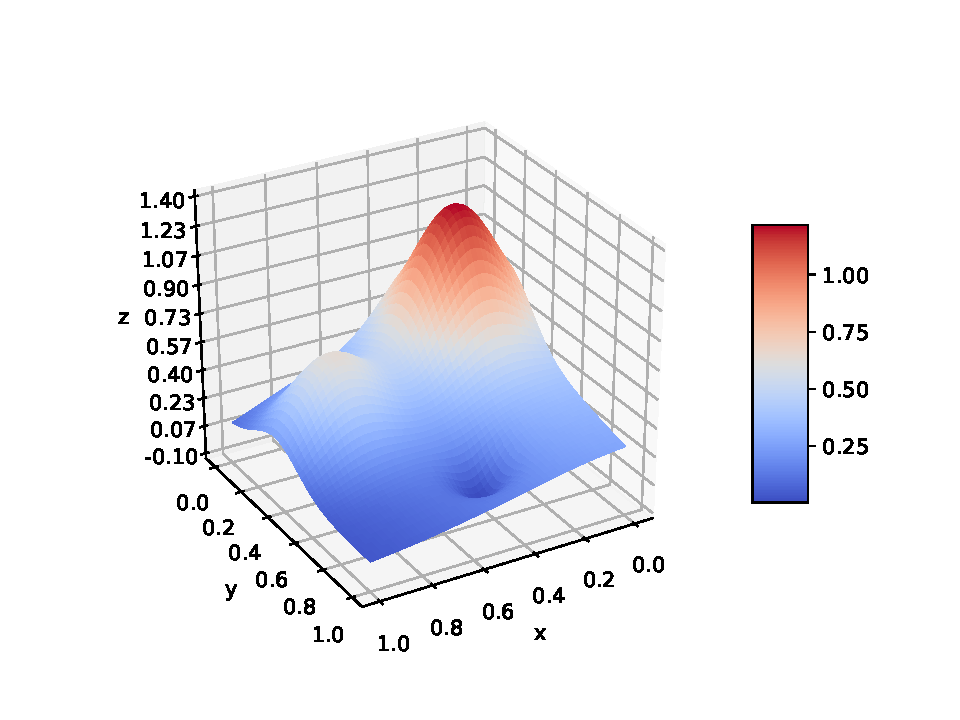
\includegraphics[width=\columnwidth]{frankefunc.pdf}
            \caption{\label{fig:FrankeFunction}The Franke Function}
        \end{figure}

\section{Results \& Discussion}

We aim to model both the Franke function and the terrain data as sums of polynomials in x and y. Our overarching goal is to determine which regression method performs the best (i.e. most faithfully reproduces the full data-set on which they are sampled) in both cases, and for which degree of the polynomial model and which value of the penalty parameter $\lambda$. The Franke function is given as in Eqn. \ref{eq:franke} over the domain $x,y \in [0,1]$.

The terrain data,  which has been downloaded from \cite{4155_repo}, is a collection of measured elevation heights at a discrete set, size $[3601,1801]$, of pixel coordinates. For ease of interpretation and computation, we parameterize the pixel indices as linearly spaced $x,y \in [0,1]$, and restrict ourselves to the first square of the terrain map, i.e. the first $[1801,1801]$ pixels.

% Below is basically a repetition of abstract/introduction, but with slightly more details.
% I don't like it, even though I wrote it. -TEM

We will first consider samplings of the Franke function. We will analyze the performance of the different regression methods for various models (polynomial degrees) and penalty parameters. We will investigate the bias-variance behaviour of the methods, and the effect of the sampling size. We will see that the addition of normally distributed noise to the sample values has a dramatic impact on the performance of the various methods. Finally we will compare various 'best predictions' for the different regression methods, in order to visualize the significance of their different approaches. These predictions will be learned on the same randomly sampled set of points in $x,y \in [0,1]$, and applied to a grid of 2000 points in each direction, with their resulting predictions being compared amongst the methods and with the ground truth of the Franke function evaluated on that grid. 

Armed with insights from the investigation of the Franke function, we will subsequently do much of the same analysis for the terrain data. Ultimately we will compare the best predictions for each method (learned on the same downsampled data set) with each other and with the ground truth of the full $[1801,1801]$ terrain map we downsampled from.

%%%The above two paragraphs could probably be cut. -TEM

\subsection{The Franke function}

    \begin{figure}[h!tb]
        \center
        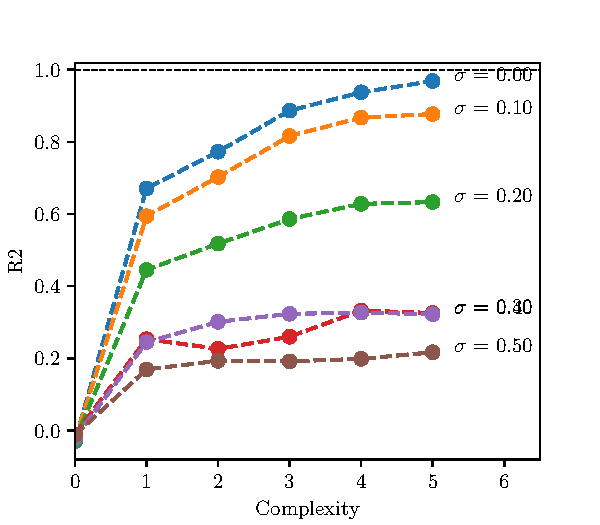
\includegraphics[width=\columnwidth]{OLS_R2_noise.pdf}
        \caption{R$^2$ measured for $N=1000$ random samples of the Franke function with added noise in the form $\delta \cdot \mathcal N(0, 1)$ modeled with complexities 0 to 5.}
    \end{figure}

    \begin{figure*}
         \centering
         \subfloat[][Ridge regression]{
            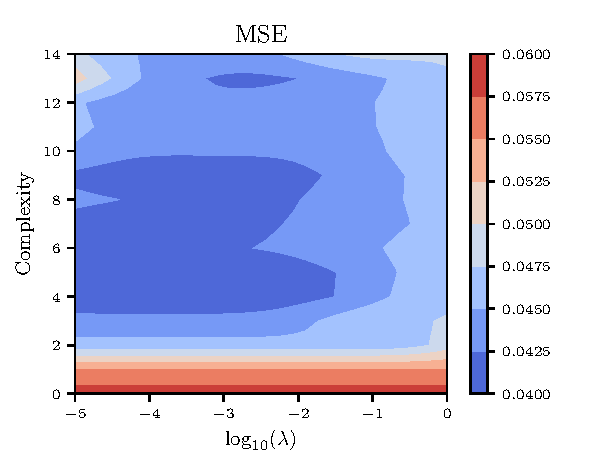
\includegraphics[width=\columnwidth]{RIDGE_CV_Franke_contour.pdf}\label{<figure1>}
         }
         \subfloat[][LASSO regression]{
            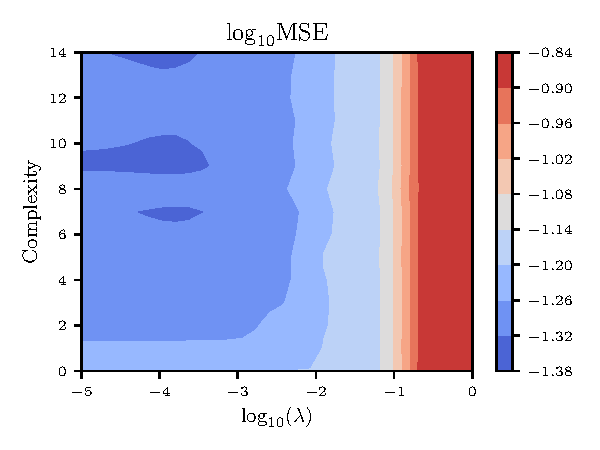
\includegraphics[width=\columnwidth]{LASSO_CV_Franke_contour.pdf}\label{<figure2>}
         }
         \caption{$\log_{10}(\textup{MSE})$ for $k=5$ crossvalidated Rige \& LASSO regression performed on $n=100$ samples of the Franke Function with added random noise in the form $0.2 \cdot \mathcal N(0, 1)$}
         \label{contour plots}
    \end{figure*}

PART A:


Subsequent parts:
%Prosjektbeskrivelsen behandler de forskjellige metodene ganske separat, og ber jo om mer eller mindre den samme typen plott tre ganger. Jeg har mest lyst til å kombinere en del av dem. For Franke tenker jeg at vi bør ha:
%
%For n=100 og for n=1000, max-degree = 20, med og uten støy
%
%- Kryssvalidert MSE for OLS og beste Ridge og beste Lasso som funksjon av polynomgrad.
%- Bootstrappet bias, varians og MSE for OLS, beste Ridge og beste lambda som funksjon av polynomgrad.
%- Predikerte plott av typen som ligger i franke_prediction_plots for beste grad (lavest MSE), og for en rimelig høy grad (med nesten like lav MSE)
%
%Da får vi allerede 4x4 = 16 plott. Vi bør kanskje ta med et par plott som viser den generelle lambda-avhengigheten, f.eks.
%
%For n=1000, max-degree = 20, med støy.
%- Kryssvalidert MSE for en håndfull Ridge-lambdaer som funksjon av polynomgrad.
%- Bootstrappet bias, varians og MSE for en håndfull Ridge-lambdaer som funksjon av polynomgrad
%- Kryssvalidert MSE for en håndfull Lasso-lambdaer som funksjon av polynomgrad.
%- Bootstrappet bias, varians og MSE for en håndfull Lasso-lambdaer som funksjon av polynomgrad.
%- Lasso og Ridge kryssvalider MSE for høyeste polynomgrad (19, siden max_degree teller med 0) og for en lavere polynomgrad (f.eks. 8), som en funksjon av lambda
%
%Da er vi oppe i 21 figurer.
%
%For terrengdataene tenker jeg:
%
%For spacing = 40 og for spacing = 100 (tilsvarer 2025 og 324 punkter), med max-degree = 20
%- Kryssvalidert MSE for OLS og beste Ridge og beste Lasso som funksjon av polynomgrad.
%- Bootstrappet MSE for OLS og beste Ridge og beste Lasso som funksjon av polynomgrad.
%-  Predikerte plott av typen som ligger i terrain_prediction_plots for beste grad (lavest MSE), og for en rimelig høy grad (som fremdeles har en rimelig lav MSE).
%
%Da får vi 2x4 plott til, og ender opp med 28 plott! I tillegg kunne jeg ha lagt til en haug som viser hvordan polynomenes MSE forandrer seg versus lambda, resultater med forskjellige lambda-intervaller og så videre for stor og liten n, stor og liten spacing, med og uten støy. Rett ut en kombinatorisk eksplosjon.
%
%Hovedhistorien, derimot, tenker jeg blir ca. som følger:
%
%Vi ser på kryssvalidert MSE for å finne beste polynomgrad. Der ser vi at de tre metodene er omtrent jevnbyrdige inntil OLS eksploderer.
%
%Av bias-varians plottet ser vi at det skjer ved at OLS får stor varians, mens ridge og lasso holder seg stabile. Vi ser at eksplosjonen skjer ved høyere grad når vi har flere punkter. Og vi ser at eksplosjonen ikke er (like mye, hvis i det hele tatt) til stede uten støy.
%
%Ved de predikerte plottene ser vi at lav polynomgrad ikke ligner særlig, selv om MSE er lav. For høy grad ser vi at OLS går dunken med støy, men klarer seg gjerne best uten støy. Vi ser at Ridge redder de høye polynomene når du har støy. Lasso ser vi at prøver å glatte ut hele plottet; ikke rart siden prediktorene våre er sterkt korrelerte.
%Vi ser at det meste blir bedre med flere punkter, og at høy polynomgrad kanskje ikke hjelper hvis man har for få datapunkter, selv med hjelp fra Ridge.
%
%Av de lambda-relaterte plottene ser vi at begge metodene kverker variansen, og ikke gir store forskjeller i MSE over et stort lambda-intervall. De største farene er ved veldig liten (numeriske feil), eller veldig stor lambda (stor effekt av penalty). Der kverker Lasso alt, og gir oss et skråplan, mens Ridge prøver å gjøre det samme uten helt å flate alt.
%
%Litt den samme karusellen gjør vi med terrengdataene. Der ser vi av de kryss-validerte MSE-ene at Lasso og Ridge stabiliserer seg som lave, selv vedhøye polynomer, mens OLS sprenges kraftig ved få punkter, og potensielt også ved mange punkter, men ved høyere polynomgrad.
%
%Av bias-varians-bootstrappen ser vi OLS mislykkes pga. varians. Da kan Ridge være til hjelp.
%
%De predikerte plottene viser at grunnen til at Ridge og Lasso gir liten MSE ved høye grader og få punkter, er at de flater ut alt. OLS er best på å gjenskape landskapets ‘ruglethet’, men kan fordreies kraftig ved få punkter.
%
%Vi ser at lav polynomgrad i alle tilfeller gjør oss ute av stand til å fange noe særlig av landskapet ruglethet. Med mange punkter kan vi gå opp til høye polynomgrader og fremdeles bruke OLS, som er mest sensitiv til landskapets variasjon. Det er likevel en risiko for at OLS prediksjonen blir fordreid, og da kan det være bedre å enten gå ned noen grader, eller bruke Ridge. Alt blir bedre med flere punkter.
%
%Oppsummert: Ikke bruk Lasso på denne typen terremgprediksjon med polynomer som basis. For god gjenskapning av terrenget trengs høy polynomgrad. Har man da ikke nok datapunkter blåser OLS opp som den store, stygge ulven i en ballongblåser-konkurrqnse. Ved ustabil OLS kan Ridge hjelpe, men går på bekostningen av detaljer i terrenget.



\subsection{The terrain data}



    \begin{figure}[h!tb]
        \center
        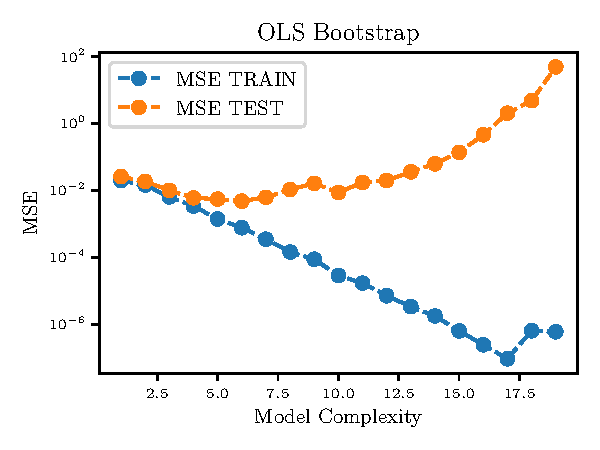
\includegraphics[width=\columnwidth]{../figs/OLS_MSE_Bootstrap_Hastie_211.pdf}
        \caption{\label{fig:Hastie2.11 MSE Bootstrap}The mean MSE for testing and training data with a 1/4 split resampled 500 times with bootstrap for a OLS regression of 300 randomly sampled points of the Franke Function.}
    \end{figure}

%\section{Discussion}

\section{Conclusion}

\onecolumngrid
\bibliography{bibfile}
\newpage
\twocolumngrid
\appendix


\end{document}
